% ─────────────────────────────────────────────────────────────────────────────
%  Paper 6 — Operationalizing Reconstructive Authority
%  Runtime Construction, Dependency Resolution, and Execution Gating
%  in Autonomous Agent Systems
%  Agent Governance Series — Paper 6 of 7
% ─────────────────────────────────────────────────────────────────────────────

\documentclass[11pt]{article}
\usepackage[utf8]{inputenc}
\usepackage[T1]{fontenc}
\usepackage{lmodern}
\usepackage[protrusion=true,expansion=false]{microtype}
\usepackage[margin=1in, top=1.1in, bottom=1.1in]{geometry}
\usepackage{amsmath,amssymb,amsthm}
\usepackage{booktabs}
\usepackage{graphicx}
\usepackage[colorlinks=true, linkcolor=blue!70!black, citecolor=blue!70!black, urlcolor=blue!70!black]{hyperref}
\usepackage{xcolor}
\usepackage{enumitem}
\usepackage[numbers,sort&compress]{natbib}
\usepackage{caption}
\captionsetup{font=small,labelfont=bf}
\usepackage{subcaption}
\usepackage{tikz}
\usetikzlibrary{shapes.geometric,arrows.meta,positioning,fit,backgrounds,calc}
\usepackage{listings}
\usepackage{float}
\usepackage{array}
\usepackage{multirow}

% ── Theorem environments ──────────────────────────────────────────────────────
\newtheorem{theorem}{Theorem}
\newtheorem{proposition}{Proposition}
\newtheorem{definition}{Definition}
\newtheorem{corollary}{Corollary}

% ── Code listing style ────────────────────────────────────────────────────────
\lstset{
  basicstyle=\small\ttfamily,
  frame=single,
  xleftmargin=1em,
  breaklines=true,
  captionpos=b
}

% ─────────────────────────────────────────────────────────────────────────────
%  TITLE & AUTHOR
% ─────────────────────────────────────────────────────────────────────────────

\title{\textbf{Operationalizing Reconstructive Authority}\\[4pt]
       \large Runtime Construction, Dependency Resolution, and Execution Gating\\
       in Autonomous Agent Systems}

\author{Marcelo Fernandez\\[2pt]
        \small TraslaIA\\[2pt]
        \small \href{https://agentcontrolprotocol.xyz}{agentcontrolprotocol.xyz}}

\date{}

\begin{document}

\maketitle

% ─────────────────────────────────────────────────────────────────────────────
%  SERIES TABLE
% ─────────────────────────────────────────────────────────────────────────────

\begin{table}[h!]
\centering
\small
\caption*{\textbf{Agent Governance Series}}
\begin{tabular}{@{}llll@{}}
\toprule
\textbf{Paper} & \textbf{Title} & \textbf{Zenodo DOI} & \textbf{arXiv} \\
\midrule
P0 & Atomic Decision Boundaries~\cite{fernandez2026a}           & 10.5281/zenodo.19670649 & 2604.17511 \\
P1 & Agent Control Protocol (ACP)~\cite{fernandez2026b}         & 10.5281/zenodo.19672575 & 2603.18829 \\
P2 & From Admission to Invariants (IML)~\cite{fernandez2026c}   & 10.5281/zenodo.19672589 & 2604.17517 \\
P3 & Fair Atomic Governance~\cite{fairgov26}                    & 10.5281/zenodo.19672597 & TBD \\
P4 & Irreducible Multi-Scale Governance~\cite{fernandez2026comp} & 10.5281/zenodo.19672608 & TBD \\
P5 & Reconstructive Authority Model (RAM)~\cite{fernandez2026ram} & 10.5281/zenodo.19669430 & TBD \\
P6 & \textbf{Operationalizing Reconstructive Authority}          & TBD & TBD \\
\bottomrule
\end{tabular}
\end{table}

% ─────────────────────────────────────────────────────────────────────────────
%  ABSTRACT
% ─────────────────────────────────────────────────────────────────────────────

\begin{abstract}
Autonomous agent systems fail not only due to incorrect decisions, but due to executing
decisions whose authority no longer holds at runtime. Prior work established that atomicity
alone cannot guarantee correct execution under dynamic conditions, and that behavioral drift
is structurally unavoidable.

In this paper, we operationalize Reconstructive Authority (RAM) as a runtime criterion for
execution: an action is permitted only if authority can be constructed from current state.
This introduces a third execution state beyond admit/deny: \textsc{halt}, representing
undefined authority due to insufficient or inconsistent observability.

We formalize RAM as a projection over state space, prove that execution without runtime
reconstruction admits inevitable failure under drift accumulation, and show that authority
is a discontinuous property with boundary sensitivity to small state perturbations.

To complete the execution model, we introduce a Recovery Loop that integrates drift
detection (IML) and execution control (ACP), enabling systems to transition from
\textsc{halt} to safe execution when observability gaps are resolved. We prove conditional
liveness: if authority-defining variables become observable, execution will eventually
resume.

The result is a unified execution model that guarantees no action is performed without
constructible authority, while maintaining progress when safety conditions can be
re-established.
\end{abstract}

\tableofcontents
\newpage

% ─────────────────────────────────────────────────────────────────────────────
\section{Introduction}
% ─────────────────────────────────────────────────────────────────────────────

Autonomous systems operate in environments where the conditions under which decisions are
made do not remain stable until execution. This gap between decision and execution is not
incidental; it is structural. Prior work in this series showed that separating evaluation
from execution introduces unavoidable inconsistencies~\cite{fernandez2026a}, that
enforcement alone cannot detect behavioral drift~\cite{fernandez2026c}, and that governance
requires multiple orthogonal layers to remain coherent under limited
observability~\cite{fernandez2026comp}.

A central failure mode emerges from this structure: systems execute decisions whose
authority no longer holds at runtime. This is not a failure of decision quality, but of
execution validity.

Reconstructive Authority (RAM), introduced in Paper~5~\cite{fernandez2026ram}, addresses
this by redefining execution as a constructibility problem: authority must be derived from
the current system state, not inherited from prior validation. However, while RAM
establishes the theoretical condition for valid execution, it does not define how such a
condition is enforced in a running system.

\textit{This paper provides that operationalization.}

We introduce a runtime execution model in which authority is evaluated at the point of
action, and execution is conditioned on its constructibility. This leads to a fundamental
extension of the execution state space: beyond traditional admit/deny outcomes, we define
a third state, \textsc{halt}, representing situations where authority cannot be established
due to incomplete or uncertain information.

The introduction of \textsc{halt} changes the nature of execution control. Systems are no
longer forced to approximate decisions under uncertainty; instead, they can explicitly
refuse to act when authority is undefined.

We further show that authority is not a continuous function of system state. Small
perturbations can invalidate execution, and sequences of decisions accumulate divergence
over time. Without runtime reconstruction, these properties guarantee eventual execution
under invalid authority.

To address this, we integrate RAM within the Agent Control Protocol
(ACP)~\cite{fernandez2026b} as the authorization criterion at the execution gate (stage~3
of the 6-stage ACP flow), and connect it with the Invariant Monitoring Layer
(IML)~\cite{fernandez2026c} for drift detection. This enables a closed-loop execution
model. ACP remains the enforcement pipeline; RAM refines its authorization semantics.

The key contribution of this paper is the introduction of a Recovery Loop that governs
system behavior after \textsc{halt}. Rather than treating \textsc{halt} as a terminal
state, the system identifies missing authority-defining variables, acquires additional
information, and attempts reconstruction. We prove that, under recoverable observability
conditions, the system will eventually resume execution.

Taken together, these elements define a complete execution model with two guarantees:

\begin{itemize}
  \item \textbf{Safety:} no action is executed without constructible authority.
  \item \textbf{Liveness:} execution resumes when authority becomes constructible.
\end{itemize}

This reframes execution in autonomous systems from a problem of estimation and validation
to one of constructibility and enforcement at runtime.

% ─────────────────────────────────────────────────────────────────────────────
\section{System Model}
% ─────────────────────────────────────────────────────────────────────────────

Let:
\begin{itemize}
  \item $S_r(t)$: real system state at time $t$
  \item $O(t) \subseteq S_r(t)$: observable state
  \item $A(t)$: execution authority
  \item $F$: authority construction function
  \item $U$: uncertainty map over state variables
\end{itemize}

Authority is defined as:
\[
  A(t) = F(S_r(t))
\]

Since $S_r(t)$ is not fully observable, the system operates on $O(t)$ and must determine
whether authority can be constructed.

\begin{definition}[Constructible Authority]
Authority is constructible at time $t$ if all variables required by $F$ can be derived
from observable and reliable state components within $O(t)$.
\end{definition}

\begin{definition}[Undefined Authority]
If any required variable is unobservable, uncertain beyond acceptable bounds, or missing,
then:
\[
  A(t) = \bot
\]
and execution must not proceed.
\end{definition}

\begin{definition}[Execution State Space]
The execution gate admits exactly three outcomes:
\[
  \mathrm{gate}(t) \in \{\textsc{execute},\; \textsc{deny},\; \textsc{halt}\}
\]
where \textsc{halt} corresponds to $A(t) = \bot$.
\end{definition}

\textbf{The \textsc{halt} state is the central innovation of this paper.} It is distinct
from \textsc{deny}:
\begin{itemize}
  \item \textsc{deny} = the system knows authority does not hold ($A(t) = \text{False}$)
  \item \textsc{halt} = the system cannot determine whether authority holds ($A(t) = \bot$)
\end{itemize}
Systems that collapse this distinction execute under undefined authority.

% ─────────────────────────────────────────────────────────────────────────────
\section{Architectural Overview}
% ─────────────────────────────────────────────────────────────────────────────

Operational RAM consists of four tightly integrated components.

\subsection{State Acquisition Layer}

Collects $O(t)$ from internal system signals, external inputs, and contextual environment.
No completeness assumption is made. Any gap in observability propagates directly to the
authority construction step.

\subsection{Authority Construction Engine}

Evaluates:
\[
  A(t) = F(O(t))
\]
via dynamic dependency resolution. The engine identifies which variables are required,
evaluates their observability and reliability, and returns one of the three authority
states.

\subsection{Execution Gate}

Enforces:
\[
  \begin{cases}
    A(t) = \text{True} & \Rightarrow \textsc{execute} \\
    A(t) = \text{False} & \Rightarrow \textsc{deny} \\
    A(t) = \bot        & \Rightarrow \textsc{halt}
  \end{cases}
\]

No execution occurs without a defined, positive authority state.

\subsection{Audit Layer}

Records for each execution attempt: the observed state $O(t)$, the dependency set $D(t)$,
the authority decision, and failure conditions. This ensures full traceability without
influencing the execution decision.

% ─────────────────────────────────────────────────────────────────────────────
\section{Runtime Authority Construction Protocol}
% ─────────────────────────────────────────────────────────────────────────────

We now define the operational protocol that implements RAM in real systems.

\subsection{Inputs}

At time $t$, the protocol receives:
\begin{itemize}
  \item Observable state $O(t)$
  \item Action class $C$
  \item Policy prior $P_0(C)$ (candidate generator only)
  \item Construction function $F$
  \item Uncertainty map $U$
\end{itemize}

\subsection{Prior Influence Constraints}

The policy prior $P_0(C)$ is strictly constrained:

\begin{itemize}
  \item It \textbf{cannot} authorize execution independently.
  \item It \textbf{cannot} override runtime construction.
  \item It \textbf{can only} propose initial candidate variables for $F$ to evaluate.
  \item Runtime construction may promote variables outside the prior when required.
  \item Demotion of required variables is not permitted within the same decision cycle
        under uncertainty.
\end{itemize}

\begin{proposition}[Prior Non-Authority]
No execution decision can be derived from $P_0(C)$ alone. Authority requires runtime
construction over $O(t)$.
\end{proposition}

\subsection{Dependency Resolution Algorithm}
\label{sec:dep-resolution}

Let $D(t)$ be the set of variables required to construct authority. The key property is:
\[
  D(t) = \mathrm{Resolve}(O(t))
\]
Dependencies are \emph{not statically defined}. They emerge from the current observable
state at runtime.

The algorithm proceeds in seven steps:

\begin{enumerate}
  \item Initialize candidate variables from $P_0(C)$.
  \item Evaluate $F$ against current state $O(t)$.
  \item Derive required dependency set $R(t)$ from actual dependencies discovered by $F$.
  \item Promote all required variables into the authority-defining set $A_d(t)$.
  \item For each variable $v \in A_d(t)$: evaluate observability and uncertainty status.
  \item If any authority-defining variable is unresolved $\Rightarrow A(t) = \bot$,
        execution halts.
  \item If all variables are resolved and constraints pass $\Rightarrow A(t) = \text{True}$,
        execution proceeds.
\end{enumerate}

\subsection{Construction Function}

\begin{lstlisting}[language=Python, caption={Runtime authority construction}]
def reconstruct_authority(state, prior):
    candidates = initialize_from_prior(prior)
    required   = resolve_dependencies(state, candidates)

    for var in required:
        if not observable(var, state):
            return UNDEFINED
        if not reliable(var, state):
            return UNDEFINED

    if not satisfies_constraints(state, required):
        return False

    return True
\end{lstlisting}

\subsection{Non-Persistence Property}

Authority is not persistent across time steps:
\[
  A(t) \neq A(t + \Delta)
\]
unless explicitly recomputed from fresh state. This property is not an engineering
limitation but a logical consequence of the reconstructive model: authority depends on
state, and state changes.

% ─────────────────────────────────────────────────────────────────────────────
\section{Drift Handling}
% ─────────────────────────────────────────────────────────────────────────────

Drift is modeled as change in $S_r(t)$ that invalidates previously held authority
components.

RAM handles drift implicitly: any change that affects $O(t)$ requires recomputation of
$A(t)$. If reconstruction fails under the new state, execution halts.

\textbf{IML integration.} Recomputation is triggered by IML anomaly signals and is
mandatory before every state-mutating action. Continuous polling is not required. This
event-driven model makes IML and RAM orthogonal and complementary: IML observes
deviations~\cite{fernandez2026c}; RAM enforces the execution consequence.

\begin{proposition}[Drift Manifestation]
Drift in $S_r(t)$ manifests as failure of authority construction. No explicit drift
detector is required for RAM to provide safety; however, IML-triggered recomputation
improves liveness by reducing unnecessary halts.
\end{proposition}

\begin{theorem}[Stale Authority Under Drift]
Any system that does not recompute authority at execution time will eventually execute
under invalid authority when $S_r(t)$ changes continuously.
\end{theorem}

\begin{proof}
Let $A(t_0) = \text{True}$ be authority computed at admission time. Let $S_r(t)$ change
continuously such that for some $t_1 > t_0$, the required variables $D(t_0)$ are no
longer valid under $S_r(t_1)$. Since authority is not recomputed, the system executes with
$A(t_1) = \text{True}$ (stale), while the correct value is $A(t_1) = \bot$ or
$A(t_1) = \text{False}$. \hfill $\blacksquare$
\end{proof}

% ─────────────────────────────────────────────────────────────────────────────
\section{Decision Model}
% ─────────────────────────────────────────────────────────────────────────────

Each execution attempt produces a deterministic decision code. The seven codes derived
from the operational protocol are:

\begin{enumerate}
  \item \texttt{ADMIT\_AUTHORITY\_CONSTRUCTIBLE} — all required variables resolved,
        constraints satisfied.
  \item \texttt{HALT\_AUTHORITY\_UNDEFINED\_REQUIRED\_DEPENDENCY} — a dependency required
        by $F$ is not observable.
  \item \texttt{HALT\_AUTHORITY\_UNDEFINED\_UNCERTAINTY} — a required variable is
        observable but uncertainty exceeds the threshold.
  \item \texttt{HALT\_MISSING\_REQUIRED\_SIGNAL} — a signal required to compute $D(t)$
        is absent.
  \item \texttt{HALT\_REATTESTATION\_REQUIRED} — authority was previously valid but state
        change mandates reconstruction before proceeding.
  \item \texttt{CONTINUE\_BOUNDED\_NON\_AUTHORITY\_DRIFT} — drift detected, but it affects
        only non-authority-defining variables; execution may proceed.
  \item \texttt{NARROW\_PRIVILEGE\_REEVALUATE} — authority partially constructible; reduce
        action scope and re-evaluate.
\end{enumerate}

\begin{proposition}[Execution Safety Invariant]
If $A(t) \neq \text{True}$, no action in execution class $C$ proceeds. This is enforced
structurally by the execution gate, not by policy configuration.
\end{proposition}

% ─────────────────────────────────────────────────────────────────────────────
\section{Auditability and Traceability}
% ─────────────────────────────────────────────────────────────────────────────

For each execution attempt, the system produces a structured audit artifact:

\begin{itemize}
  \item Timestamp and action identifier.
  \item Initial prior candidates from $P_0(C)$.
  \item Runtime required set $R(t)$ with discovery path.
  \item Promotions into $A_d(t)$ with reason.
  \item Uncertainty status $U(v)$ for each authority-defining variable.
  \item Final decision code and halt or continue rationale.
\end{itemize}

The audit artifact explains not only the decision, but why specific variables became
authority-defining and how they affected the outcome. This enables post-hoc analysis,
regulatory compliance, and system validation without influencing execution behavior.

% ─────────────────────────────────────────────────────────────────────────────
\section{Integration with the Governance Stack}
% ─────────────────────────────────────────────────────────────────────────────

RAM does not replace any existing governance layer. It operates as the authorization
criterion within the execution gate of ACP (stage~3 of the 6-stage ACP enforcement
flow). Each layer retains its distinct role:

\subsection{Atomic Execution (Paper~0)}

Paper~0~\cite{fernandez2026a} establishes that decision and action must be atomically
bound to eliminate TOCTOU vulnerabilities. RAM operates within this atomicity guarantee:
the authority construction and the execution it authorizes are part of the same atomic
unit.

\subsection{Enforcement Layer (ACP, Paper~1)}

ACP~\cite{fernandez2026b} provides the enforcement pipeline: capability scoping,
constraint validation, and execution control across 6 stages. RAM replaces the
admission-time authorization criterion at stage~3 with a runtime constructibility check.
ACP remains the pipeline; RAM refines its authorization semantics without altering the
pipeline structure.

\subsection{Behavioral Layer (IML, Paper~2)}

IML~\cite{fernandez2026c} detects behavioral drift and non-identifiability. In the
integrated model, IML anomaly signals trigger RAM recomputation. This event-driven
coupling ensures that authority is reconstructed when the governance stack observes
meaningful state changes, without requiring continuous polling.

\subsection{Allocation Layer (Paper~3)}

Paper~3~\cite{fairgov26} determines which agents are permitted to reach the execution
gate. RAM determines whether execution is valid once an agent has been allocated access.
The two layers are orthogonal: allocation controls who arrives; RAM controls what executes.

\subsection{Compositional Governance (Paper~4)}

Paper~4~\cite{fernandez2026comp} establishes that the four governance dimensions are
irreducible. RAM becomes the terminal execution condition across all governance scales,
ensuring that compositional correctness at the structural level does not substitute for
runtime constructibility.

\subsection{Reconstructive Authority Model (Paper~5)}

Paper~5~\cite{fernandez2026ram} defines the formal model that this paper operationalizes.
The relationship is the same as between GAT (Paper~0) and ACP (Paper~1): the theory
defines what must hold; the operationalization defines how it is enforced.

% ─────────────────────────────────────────────────────────────────────────────
\section{Recovery Loop under Reconstructive Authority}
% ─────────────────────────────────────────────────────────────────────────────

The introduction of the \textsc{halt} state ($A(t) = \bot$) ensures that execution does
not proceed under undefined authority. However, safe systems must also provide a mechanism
to recover from \textsc{halt} when the underlying cause is resolvable.

We define the Recovery Loop as the closed process that transitions the system from
\textsc{halt} to a state where authority may be reconstructible again.

\subsection{HALT Semantics}

A \textsc{halt} occurs when:
\[
  A(t) = F(S_r(t)) = \bot
\]

This may result from:
\begin{itemize}
  \item Missing required signals
  \item Authority-defining uncertainty exceeding resolution bounds
  \item Drift invalidating prior authority assumptions
\end{itemize}

\textsc{halt} is not a terminal failure, but a controlled suspension of execution.

\subsection{Recovery Loop Definition}

Let $t$ be the time of \textsc{halt}. The system enters a recovery process:
\[
  S_r(t) \rightarrow S_r(t') \rightarrow S_r(t'')
\]
through the following stages:

\begin{enumerate}
  \item \textbf{Signal Extraction.}
        Identify the minimal set of unresolved variables $U(t)$ responsible for
        $A(t) = \bot$.

  \item \textbf{IML Trigger.}
        The IML layer~\cite{fernandez2026c} detects drift or observability gaps and emits
        a recovery trigger, directing the state acquisition layer to focus on the
        identified gap.

  \item \textbf{State Augmentation.}
        Acquire additional observations or reduce action scope:
        \[
          S_r(t') = S_r(t) \cup \Delta O
        \]
        If state augmentation cannot resolve the unobservable variables, the system may
        revert to the last atomically consistent state as established by
        Paper~0~\cite{fernandez2026a}, preserving execution integrity without requiring
        complete observability recovery.

  \item \textbf{Reconstruction Attempt.}
        Recompute authority from augmented state:
        \[
          A(t') = F(S_r(t'))
        \]

  \item \textbf{Resolution.}
        \begin{itemize}
          \item If $A(t') \neq \bot$ $\Rightarrow$ execution resumes
          \item If $A(t') = \bot$ $\Rightarrow$ remain in \textsc{halt} or escalate
        \end{itemize}
\end{enumerate}

\subsection{Integration with ACP}

The Recovery Loop operates within the execution gate of ACP:

\begin{itemize}
  \item ACP provides the execution pipeline and enforcement structure.
  \item RAM defines the authorization criterion at the gate.
  \item IML provides drift detection and recovery triggers.
\end{itemize}

Thus, RAM does not replace ACP, but refines its authorization semantics. The Recovery Loop
closes the loop between all three layers: IML $\rightarrow$ RAM $\rightarrow$ ACP
$\rightarrow$ IML.

\begin{theorem}[Conditional Liveness under Recoverable Observability]
\label{thm:liveness}
If all authority-defining variables required by $F$ are eventually observable or
resolvable, then a system implementing the Recovery Loop will eventually exit
\textsc{halt} and resume execution.
\end{theorem}

\begin{proof}
Assume a \textsc{halt} at time $t$ such that $A(t) = \bot$.
Let $U(t)$ be the set of unresolved authority-defining variables.

By assumption, each variable in $U(t)$ becomes observable or resolvable at some future
time through state augmentation:
\[
  S_r(t) \rightarrow S_r(t') \rightarrow S_r(t'')
\]
such that $U(t'') = \emptyset$.

Then:
\[
  F(S_r(t'')) = \text{True} \;\Rightarrow\; A(t'') \neq \bot
\]

Thus, execution resumes. \textsc{halt} is not terminal when observability gaps are
recoverable; the system guarantees eventual progress. \hfill $\blacksquare$
\end{proof}

% ─────────────────────────────────────────────────────────────────────────────
\section{Comparative Analysis}
% ─────────────────────────────────────────────────────────────────────────────

We situate RAM operationalization against existing execution control paradigms.

\subsection{Attestation-Based Systems}

Attestation systems~\cite{costan2016intel,sabt2015trusted} verify integrity of the
execution environment at initialization. They assume completeness: if the initial state
is valid, execution is valid. Under dynamic conditions this assumption fails; authority
derived from initial attestation may not hold at execution time.

\subsection{Risk-Threshold Systems}

Risk-gated systems~\cite{greenblatt2024ai,leike2018ai} bound uncertainty and execute
under ``acceptable risk.'' This conflates bounded uncertainty with constructible authority.
RAM rejects this: partial observability that affects authority-defining variables produces
$A(t) = \bot$ regardless of the magnitude of uncertainty.

\subsection{Reconstructive Systems}

RAM-based systems require construction of authority from current state before every
action. Any unresolved dependency collapses authority to undefined, preventing execution.

\begin{theorem}[Authority Validity]
\label{thm:validity}
Any system that permits execution under incomplete authority-defining state cannot
guarantee that no action proceeds without constructible authority.
\end{theorem}

\begin{proof}
Let a system $\mathcal{S}$ permit execution when $D(t) \not\subseteq O(t)$ for some
required set $D(t)$. Then there exists an execution at time $t$ where $A(t) = \bot$ (by
Definition~2) yet $\mathcal{S}$ proceeds. This violates the execution safety invariant
(Proposition~3). RAM satisfies it by construction through the dependency resolution
algorithm (Section~\ref{sec:dep-resolution}). \hfill $\blacksquare$
\end{proof}

% ─────────────────────────────────────────────────────────────────────────────
\section{Trade-offs}
% ─────────────────────────────────────────────────────────────────────────────

\subsection{Advantages}

\begin{itemize}
  \item \textbf{Safety guarantee:} no action proceeds without constructible authority.
  \item \textbf{Full traceability:} every decision is explained by the audit artifact.
  \item \textbf{Deterministic gating:} outcomes are computable, not probabilistic.
  \item \textbf{Liveness:} Recovery Loop ensures the system resumes when conditions allow.
\end{itemize}

\subsection{Costs}

\begin{itemize}
  \item \textbf{Increased halting frequency:} partial observability produces more
        \textsc{halt} events than threshold-based systems.
  \item \textbf{Higher latency:} recomputation at every execution step adds overhead.
  \item \textbf{Dependence on observability:} liveness is conditional on the eventual
        recoverability of required signals.
\end{itemize}

These costs are the direct consequence of choosing correctness over availability. In
safety-critical systems this trade-off is appropriate: halting is always preferable to
acting without constructible authority.

% ─────────────────────────────────────────────────────────────────────────────
\section{Conclusion}
% ─────────────────────────────────────────────────────────────────────────────

Operationalizing reconstructive authority requires four shifts:

\begin{enumerate}
  \item From validation to \textbf{construction} --- authority must be built from current
        state, not inherited.
  \item From persistence to \textbf{recomputation} --- authority expires with the state
        that produced it.
  \item From risk acceptance to \textbf{execution refusal} --- undefined authority
        mandates \textsc{halt}.
  \item From stopping to \textbf{recovery} --- \textsc{halt} triggers a closed loop that
        attempts to restore constructibility.
\end{enumerate}

Together, Papers~5 and~6 complete the governance series:

\begin{itemize}
  \item Papers~0--4 define the conditions under which governance is structurally sound.
  \item Paper~5 defines what authority must be.
  \item Paper~6 defines how authority is enforced at runtime.
\end{itemize}

The result is a system with two formal properties: \textbf{safety} (no action without
constructible authority, Theorems~\ref{thm:validity} and~\ref{thm:liveness}) and
\textbf{liveness} (execution resumes when observability is recoverable,
Theorem~\ref{thm:liveness}).

\medskip
\noindent\textit{Execution authority is not inherited. It is not validated. It is
constructed. When it cannot be constructed, execution must not occur.}

% ─────────────────────────────────────────────────────────────────────────────
%  FIGURES
% ─────────────────────────────────────────────────────────────────────────────

\newpage

% ── Figure 1 — Runtime Authority Construction Flow ───────────────────────────
\begin{figure}[H]
\centering
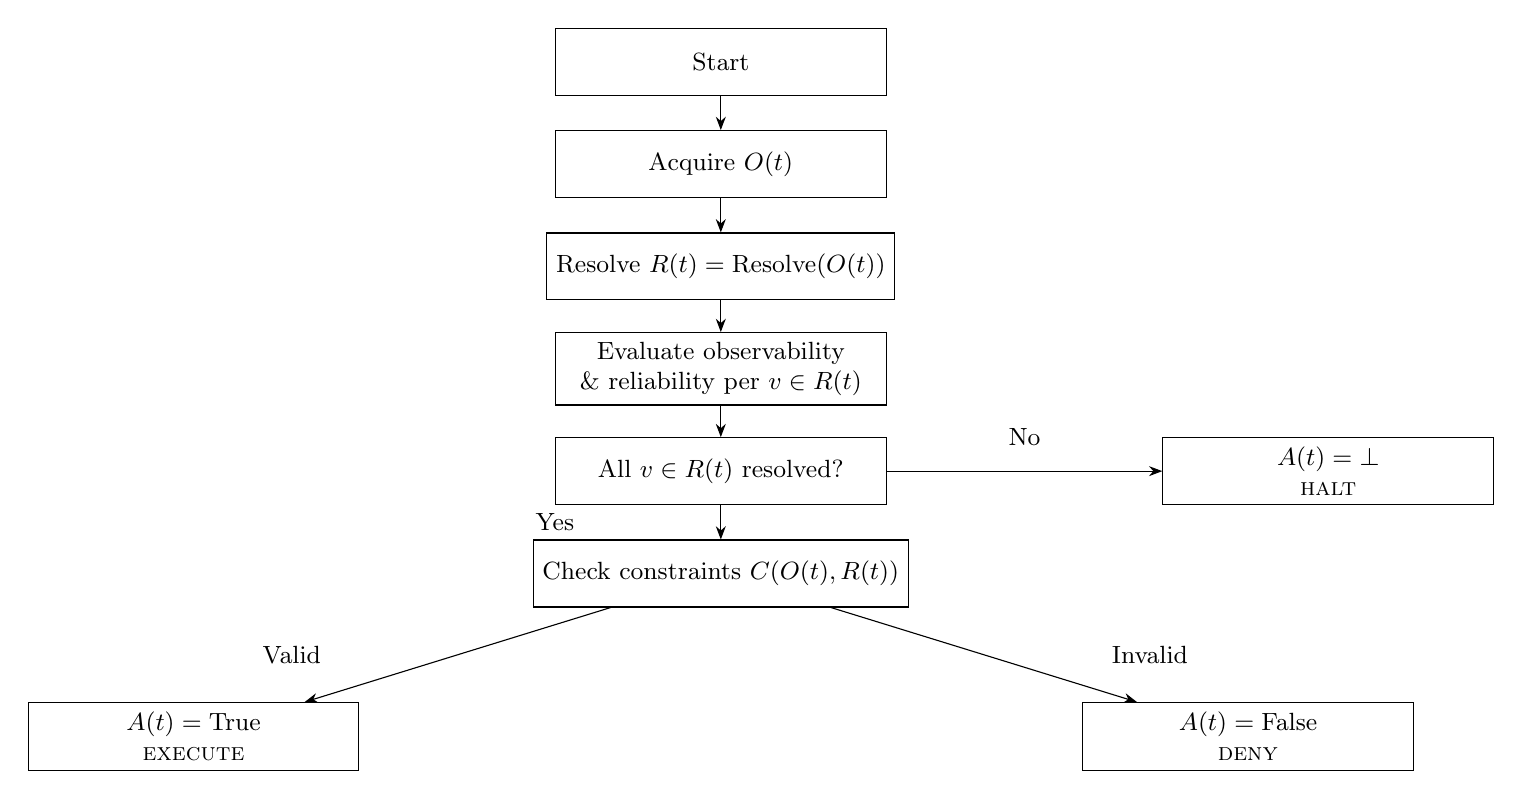
\begin{tikzpicture}[
  >=Stealth,
  node distance=1.3cm,
  every node/.style={draw, rectangle, align=center,
                     minimum width=4.2cm, minimum height=0.85cm, font=\small}
]
\node (start)       {Start};
\node (obs)         [below of=start]  {Acquire $O(t)$};
\node (dep)         [below of=obs]    {Resolve $R(t) = \mathrm{Resolve}(O(t))$};
\node (eval)        [below of=dep]    {Evaluate observability \\ \& reliability per $v \in R(t)$};
\node (check)       [below of=eval]   {All $v \in R(t)$ resolved?};
\node (constraints) [below of=check]  {Check constraints $C(O(t), R(t))$};

\node (exec) [below left=1.2cm and 2.2cm of constraints]  {$A(t)=\text{True}$ \\ \textsc{execute}};
\node (deny) [below right=1.2cm and 2.2cm of constraints] {$A(t)=\text{False}$ \\ \textsc{deny}};
\node (halt) [right=3.5cm of check]                       {$A(t)=\bot$ \\ \textsc{halt}};

\draw[->] (start) -- (obs);
\draw[->] (obs)   -- (dep);
\draw[->] (dep)   -- (eval);
\draw[->] (eval)  -- (check);
\draw[->] (check) -- node[left,draw=none]{Yes} (constraints);
\draw[->] (check) -- node[above,draw=none]{No}  (halt);
\draw[->] (constraints) -- node[left,draw=none]{Valid}   (exec);
\draw[->] (constraints) -- node[right,draw=none]{Invalid} (deny);
\end{tikzpicture}
\caption{Runtime authority construction flow. Execution proceeds only if authority can
         be constructed from current state. Unresolved dependencies collapse the decision
         to \textsc{halt}.}
\label{fig:flow}
\end{figure}

% ── Figure 2 — Dynamic Dependency Resolution ─────────────────────────────────
\begin{figure}[H]
\centering
\begin{tikzpicture}[
  >=Stealth,
  node distance=1.5cm,
  every node/.style={draw, rectangle, align=center,
                     minimum width=2.8cm, minimum height=0.8cm, font=\small}
]
\node (state) {$O(t)$};

\node (x1) [below left=1.2cm and 1.5cm of state]  {$x_1$};
\node (x2) [below=1.2cm of state]                  {$x_2$};
\node (x3) [below right=1.2cm and 1.5cm of state]  {$x_3$};

\node (F)    [below=1.2cm of x2, minimum width=3.8cm] {Construction Function $F$ \\ $\Rightarrow R(t)$};
\node (auth) [below=1.2cm of F,  minimum width=3.8cm] {Authority $A(t)$};

\draw[->] (state) -- (x1);
\draw[->] (state) -- (x2);
\draw[->] (state) -- (x3);
\draw[->] (x1) -- (F);
\draw[->] (x2) -- (F);
\draw[->] (x3) -- (F);
\draw[->] (F)  -- (auth);
\end{tikzpicture}
\caption{Dynamic dependency resolution. Authority is constructed from runtime-discovered
         dependencies over observable state. Dependencies emerge from $F$, not from a
         static definition.}
\label{fig:deps}
\end{figure}

% ── Figure 3 — Full RAM Protocol Diagram ─────────────────────────────────────
\begin{figure*}[t]
\centering
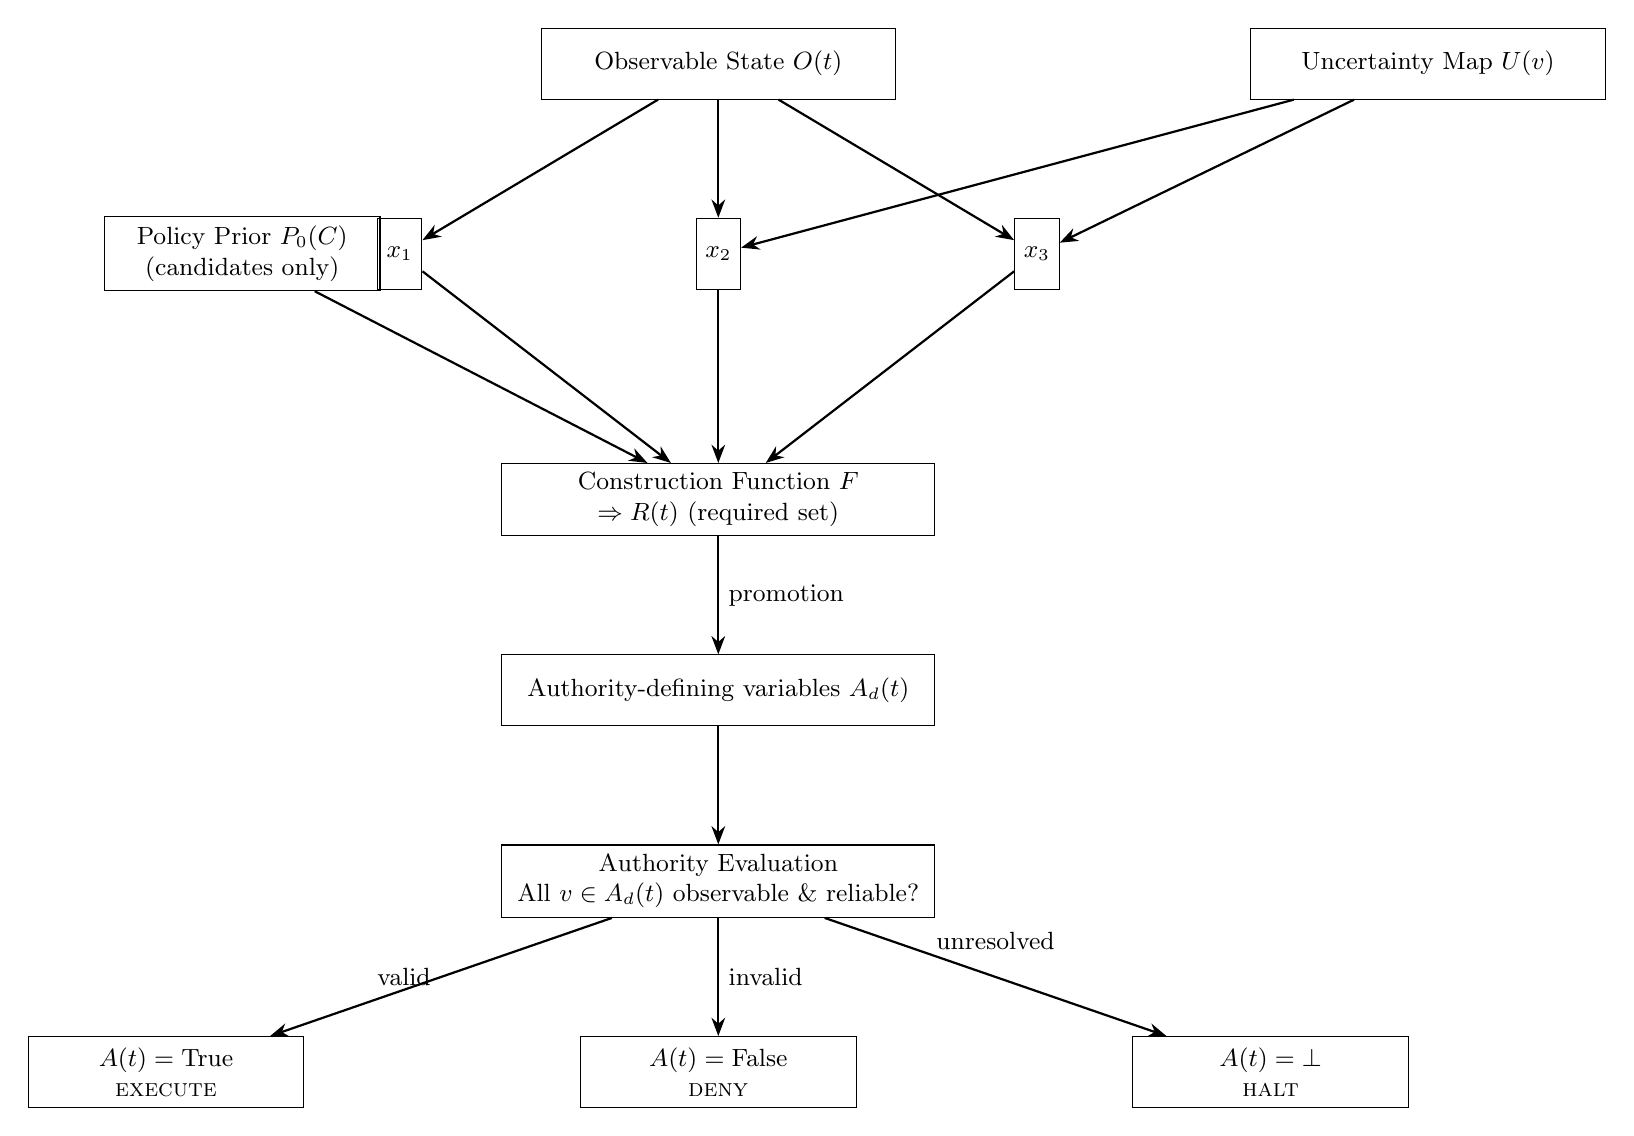
\begin{tikzpicture}[
  >=Stealth,
  node distance=1.8cm,
  every node/.style={draw, rectangle, align=center, minimum height=0.9cm, font=\small},
  arrow/.style={->, thick}
]
% STATE LAYER
\node (state)  [minimum width=4.5cm] {Observable State $O(t)$};
\node (uncert) [right=4.5cm of state, minimum width=4.5cm] {Uncertainty Map $U(v)$};

% VARIABLE NODES
\node (x1) [below left=1.5cm and 1.5cm of state]  {$x_1$};
\node (x2) [below=1.5cm of state]                  {$x_2$};
\node (x3) [below right=1.5cm and 1.5cm of state]  {$x_3$};

\node (prior) [left=4cm of x2, minimum width=3.5cm]
              {Policy Prior $P_0(C)$ \\ (candidates only)};

% CONSTRUCTION
\node (F) [below=2.2cm of x2, minimum width=5.5cm]
          {Construction Function $F$ \\ $\Rightarrow R(t)$ (required set)};

% AUTHORITY SET
\node (authset) [below=1.5cm of F, minimum width=5.5cm]
                {Authority-defining variables $A_d(t)$};

% GATE
\node (gate) [below=1.5cm of authset, minimum width=5.5cm]
             {Authority Evaluation \\ All $v \in A_d(t)$ observable \& reliable?};

% OUTCOMES
\node (exec) [below left=1.5cm and 2.5cm of gate,  minimum width=3.5cm]
             {$A(t)=\text{True}$ \\ \textsc{execute}};
\node (deny) [below=1.5cm of gate,                  minimum width=3.5cm]
             {$A(t)=\text{False}$ \\ \textsc{deny}};
\node (halt) [below right=1.5cm and 2.5cm of gate,  minimum width=3.5cm]
             {$A(t)=\bot$ \\ \textsc{halt}};

\draw[arrow] (state)   -- (x1);
\draw[arrow] (state)   -- (x2);
\draw[arrow] (state)   -- (x3);
\draw[arrow] (prior)   -- (F);
\draw[arrow] (x1)      -- (F);
\draw[arrow] (x2)      -- (F);
\draw[arrow] (x3)      -- (F);
\draw[arrow] (uncert)  -- (x3);
\draw[arrow] (uncert)  -- (x2);
\draw[arrow] (F)       -- node[right,draw=none]{promotion} (authset);
\draw[arrow] (authset) -- (gate);
\draw[arrow] (gate)    -- node[left,draw=none]{valid}      (exec);
\draw[arrow] (gate)    -- node[right,draw=none]{invalid}   (deny);
\draw[arrow] (gate)    -- node[above,draw=none]{unresolved}(halt);
\end{tikzpicture}
\caption{Full RAM protocol diagram. Observable state $O(t)$ and uncertainty $U(v)$ feed
         dynamic dependency resolution through $F$, producing the required set $R(t)$ and
         authority-defining variables $A_d(t)$. Execution proceeds only if all required
         variables are observable and reliable. Policy prior $P_0(C)$ contributes
         candidates but cannot authorize execution independently.}
\label{fig:fullram}
\end{figure*}

% ── Figure 4 — Multi-Layer Governance Stack ───────────────────────────────────
\begin{figure*}[t]
\centering
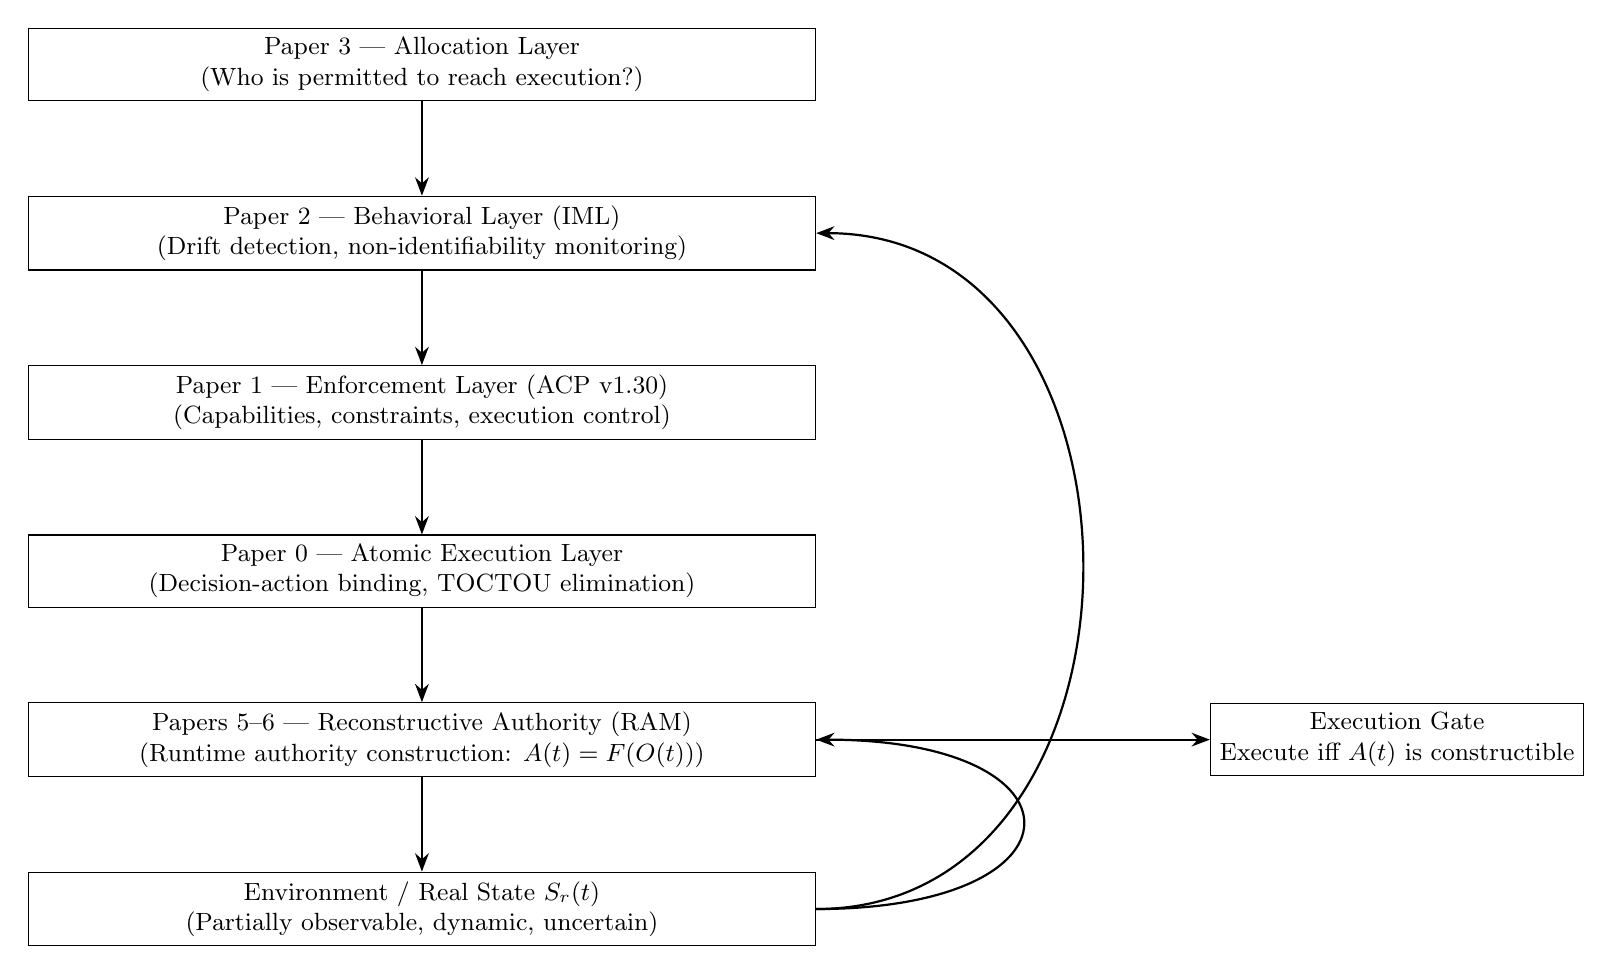
\begin{tikzpicture}[
  >=Stealth,
  node distance=1.2cm,
  every node/.style={draw, rectangle, align=center,
                     minimum width=10cm, minimum height=0.9cm, font=\small},
  arrow/.style={->, thick}
]
\node (alloc)  {Paper 3 --- Allocation Layer \\ (Who is permitted to reach execution?)};
\node (iml)    [below=of alloc]  {Paper 2 --- Behavioral Layer (IML) \\ (Drift detection, non-identifiability monitoring)};
\node (acp)    [below=of iml]    {Paper 1 --- Enforcement Layer (ACP v1.30) \\ (Capabilities, constraints, execution control)};
\node (atomic) [below=of acp]    {Paper 0 --- Atomic Execution Layer \\ (Decision-action binding, TOCTOU elimination)};
\node (ram)    [below=of atomic] {Papers 5--6 --- Reconstructive Authority (RAM) \\ (Runtime authority construction: $A(t) = F(O(t))$)};
\node (env)    [below=of ram]    {Environment / Real State $S_r(t)$ \\ (Partially observable, dynamic, uncertain)};

\draw[arrow] (alloc)  -- (iml);
\draw[arrow] (iml)    -- (acp);
\draw[arrow] (acp)    -- (atomic);
\draw[arrow] (atomic) -- (ram);
\draw[arrow] (ram)    -- (env);

% Feedback loops
\draw[arrow] (env.east) .. controls +(3.5,0) and +(3.5,0) .. (ram.east);
\draw[arrow] (env.east) .. controls +(4.5,0) and +(4.5,0) .. (iml.east);

% Execution gate annotation
\node (gate) [right=5cm of ram, minimum width=4.5cm, draw]
             {Execution Gate \\ Execute iff $A(t)$ is constructible};
\draw[arrow] (ram) -- (gate);
\end{tikzpicture}
\caption{Multi-layer governance stack integrating Papers~0--5 with runtime reconstructive
         authority (Paper~6). Allocation controls access, IML detects drift, ACP enforces
         constraints, atomic execution ensures decision binding, and RAM determines whether
         execution is valid at runtime. The environment continuously feeds state back into
         the system, requiring authority to be reconstructed before every action.}
\label{fig:stack}
\end{figure*}

% ── Figure 5 — Recovery Loop Dynamics ────────────────────────────────────────
\begin{figure}[H]
\centering
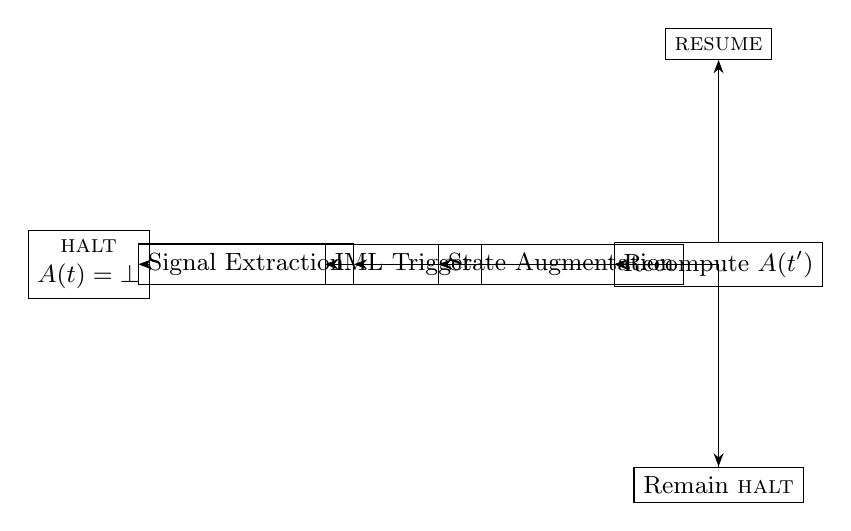
\begin{tikzpicture}[
  >=Stealth,
  node distance=2cm,
  every node/.style={font=\small}
]
\node (halt)       [draw, rectangle, align=center] {\textsc{halt} \\ $A(t)=\bot$};
\node (signal)     [draw, rectangle, right of=halt]       {Signal Extraction};
\node (trigger)    [draw, rectangle, right of=signal]     {IML Trigger};
\node (augment)    [draw, rectangle, right of=trigger]    {State Augmentation};
\node (reconstruct)[draw, rectangle, right of=augment]    {Recompute $A(t')$};

\node (resume) [draw, rectangle, above of=reconstruct, yshift=0.8cm]
               {\textsc{resume}};
\node (remain) [draw, rectangle, below of=reconstruct, yshift=-0.8cm]
               {Remain \textsc{halt}};

\draw[->] (halt)        -- (signal);
\draw[->] (signal)      -- (trigger);
\draw[->] (trigger)     -- (augment);
\draw[->] (augment)     -- (reconstruct);
\draw[->] (reconstruct) -- (resume);
\draw[->] (reconstruct) -- (remain);
\draw[->] (remain)      |- (signal);
\end{tikzpicture}
\caption{Recovery Loop under RAM. Upon \textsc{halt}, the system identifies missing
         authority components, triggers re-evaluation via IML, augments state (or reverts
         to the last atomically consistent state per Paper~0), and attempts
         reconstruction. Execution resumes only if authority becomes constructible;
         otherwise the system remains in \textsc{halt}.}
\label{fig:recovery}
\end{figure}

% ─────────────────────────────────────────────────────────────────────────────
%  BIBLIOGRAPHY
% ─────────────────────────────────────────────────────────────────────────────

\bibliographystyle{plainnat}
\bibliography{references}

\end{document}
